\chapter{Measuring platform}

The method of shunt resistor was chosen to measure the energy consumption of the GPS system. The shunt resistor was chosen due to its low complexity compared to the Hall effect IC.  The other software estimation techniques and cycle aware techniques was not chosen, as they either tries to estimate the energy consumption with poor accuracy or they need non available RTL information about the design. The shunt resistor threats the system that is getting measured as a black box, which enables the measuring platform to be used with any system. Two configurations of the measurement platform with a shunt resistor was developed. This section will explain the functionality of each component of the measurement platfrom.


\section{PicoScope 640 AD}
PicoScope 6000 from Picotecnology is a 4 channel digital oscilloscope with 5GS/s sampling and 2 GSample buffer memory \cite{Pico}. The oscilloscope is equipped with USB 3.0 and supplied with an SDK that enables the user to write their own software. The PicoScope has advanced trigger possibilities and a bandwidth of 500MHz along with a signal generator. The oscilloscope is used to measure the voltage drop across the shunt resistor.   

\section{PC with python script}
A Python API that uses the SDK from Picoscope is executed on the PC. The script is a modified version of the framework by Amen Hussain \cite{Amen}. The script is included in the appendix \ref{Appendix:EnergyMeasure.py}. The script measures the voltage drop over the shunt resistor by using the following parameters:

\begin{itemize}
    \item sampling- The sampling frequency 
    \item duration- The length of each waveform
    
\end{itemize}
The sampling and duration is used to generate a waveform of the sampled data.
The sequence diagram in figure \ref{fig:sequence} shows the interaction between the python script and the oscilloscope.  

\begin{figure}[H]
\centering
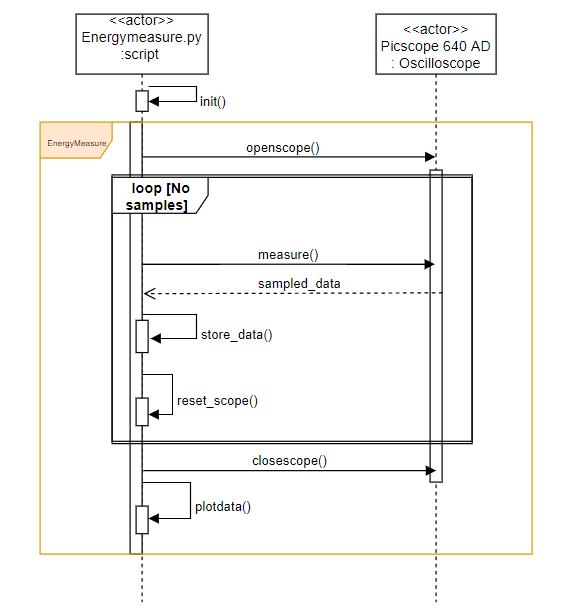
\includegraphics[height=10.5cm]{Project_Report/Images/Sequence_diagram.PNG}
\caption{Sequence diagram for the measurement script}
\label{fig:sequence}
\end{figure}
 

 The script samples the data and stores it in a list, before it restarts the sampling for the next waveform. An overhead of storing data and initializing the oscilloscope before each sample introduces a limit for the processing speed of the measurements. The measured delay caused by the overhead in software is 20-50 milliseconds between each waveform. The delay is found by using timers in software during the execution of the python script. This means that some data is not captured during the overhead process and constrains the accuracy of the measurements.
The Python script generates a plot of each waveform after the data has been analyzed \ref{fig:pythonwaveform}

\begin{figure}[H]
\centering
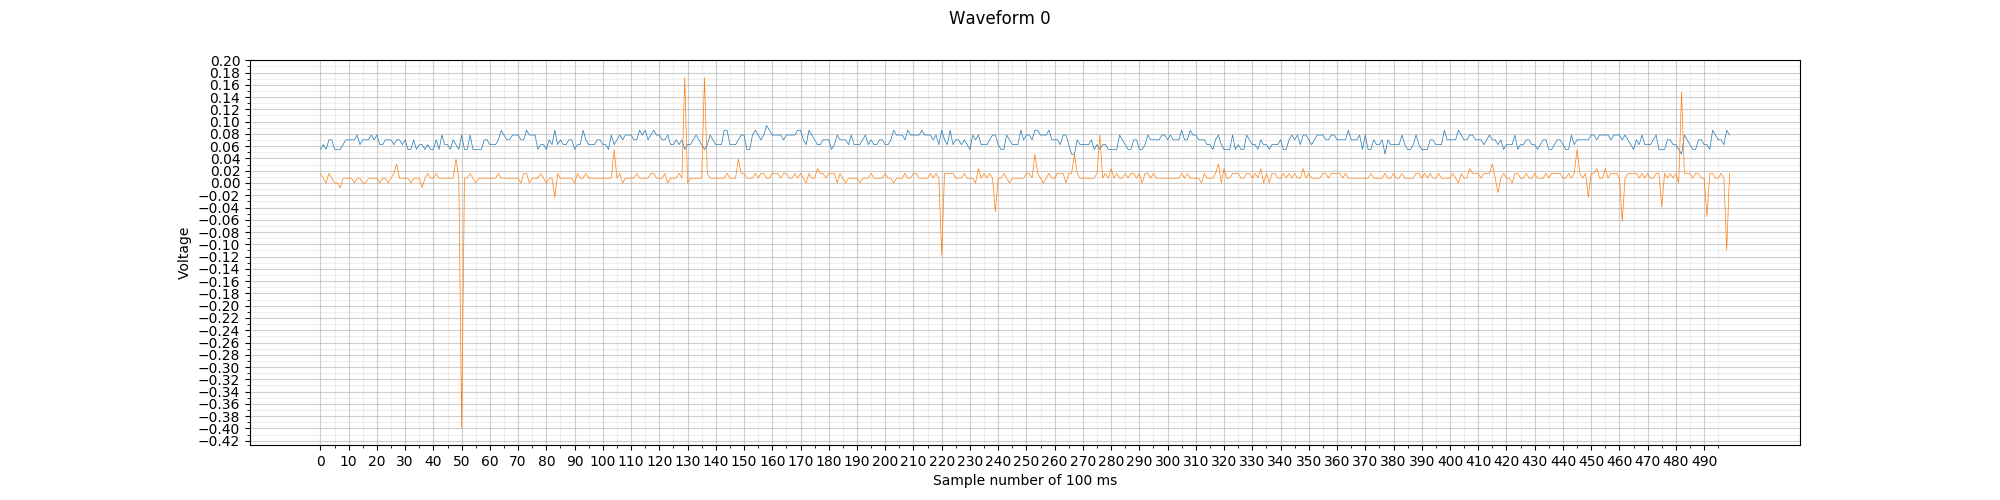
\includegraphics[height=4.5cm]{Project_Report/Images/pythonwaveform.png}
\caption{The waveform that is plotted by the python script and used for analyzing the current consumption}
\label{fig:pythonwaveform}
\end{figure}
 
An Excel document with the average current and power of each waveform is also generated. Figure \ref{fig:waveexcel} shows a screenshot of the generated excel spreadsheet for 13 waveforms.

\begin{figure}[H]
\centering
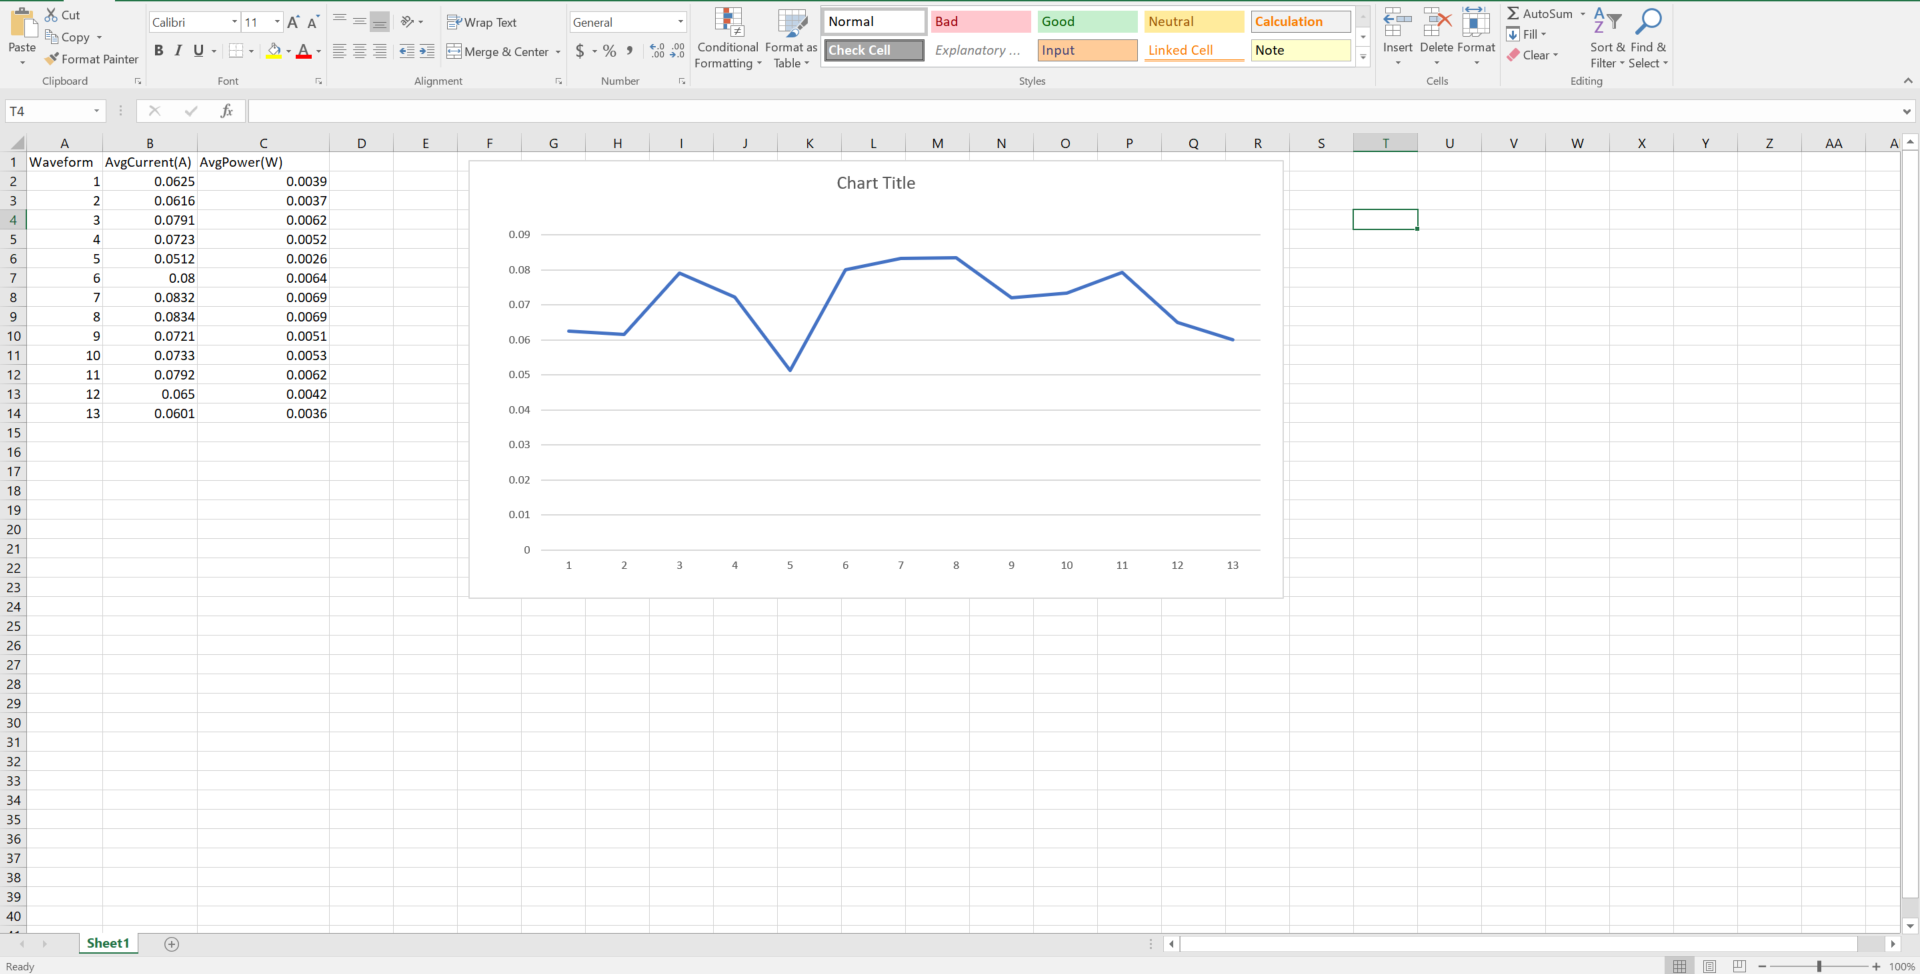
\includegraphics[height=8.0cm]{Project_Report/Images/waveformexcel.PNG}
\caption{Spreedsheet with the average current of 13 waveforms}
\label{fig:waveexcel}
\end{figure}
 



\section{Configuration options}
 Two configurations of the measurement platform with shunt resistor was developed. The first used a C027 application board from u-blox, while the other used a LoPy microcontroller from PyCom. Both methods used the PC and the Oscilloscope. 
 


\subsection{Configuration with C027}
Figure \ref{fig:deploy_C027} shows the deployment diagram of the configuration with the C027 development kit.  

\begin{figure}[H]
\centering
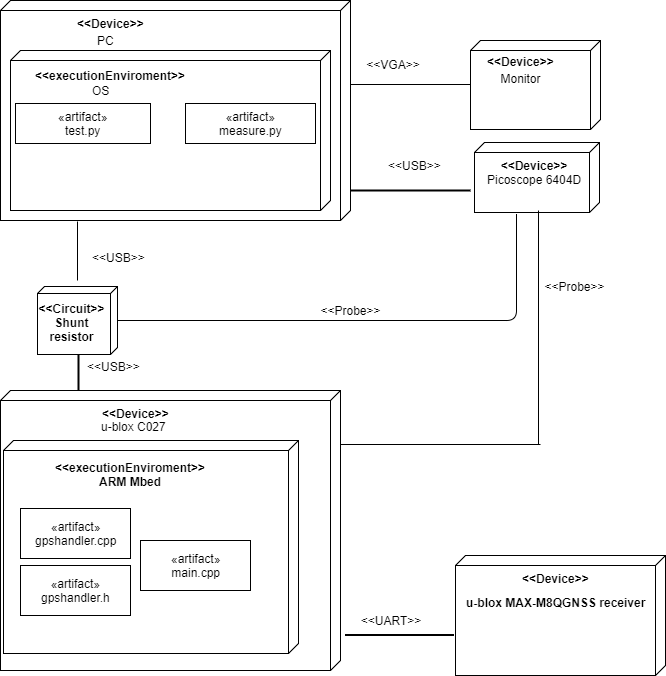
\includegraphics[height=9.5cm]{Project_Report/Images/C027_deploy.png}
\caption{Deployment diagram of the configuration with the C027}
\label{fig:deploy_C027}
\end{figure}
\vspace{5mm}The u-blox C027 is a development board for IoT applications that supports GSM, UMTS and CDMA networks. The development board has a MAX-M8Q GNSS receiver and a cellular module. The header connector has 6 analog inputs, 9 PWM, 22 GPIO, 1 SPI, 1 I2C, 1 UART and 1 I2S. C027 is supported by ARM Mbed, which is an operating system for IoT devices \cite{C027}. The application board has no embedded low power mode, but some peripherals like the GPS can be turned off with UART. Time to first fix (TTFF) for the receiver is \cite{MAX-M8}:
\begin{itemize}
    \item Cold start: 30s
    \item Hot  start: 1s
\end{itemize}

Two threads are run in "main.cpp" on the C027, the first thread receives the requested command from the PC and updates a shared variable between the two threads. The value of the shared variable corresponds to a predefined action. The second thread checks the value of the shared variable and executes the action by sending a certain sequence of bits over UART to the GPS. At the same time the action is executed, a GPIO pin is pulled high to signalize to the PC that a measurement should be done. The code that was written for C027 is included in the appendix \ref{Appendix:C027.Cpp}. 

To measure the current consumption of the application board, we had to put the shunt resistor between the VCC and GND from the USB connection. The VCC for the USB connection could not be sinked from the USB port, because the value of the VCC would not be constant 5v and therefore introduce an error to the measurement. We decided therefore to use a 12 V battery and the LM317 voltage regulator for producing the VCC for the application board. Figure \ref{fig:Schematic_C027} shows the schematic of the C027 configuration with the LM317 voltage regulator. 

\begin{figure}[H]
\centering
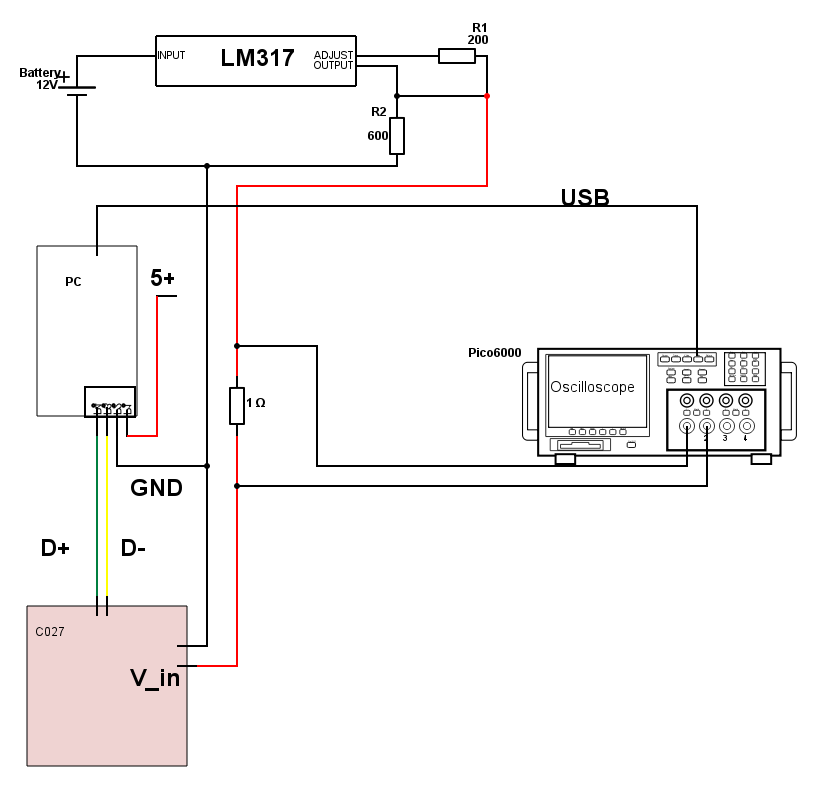
\includegraphics[height=6.5cm]{Project_Report/Images/C027_Schematic.png}
\caption{Schematic of the C027 configuration}
\label{fig:Schematic_C027}
\end{figure}

The oscilloscope measures the voltage after shunt resistor. The voltage drop over the shunt resistor is estimated by first measuring the output of the voltage regulator, and then measuring the voltage after the shunt resistor and subtracting them in software. Measuring the voltage drop directly will change the common ground for the oscilloscope, C027 and the PC to the node after the shunt resistor. This is undesired, because it prevents the oscilloscope from measuring another signal which is not referenced to that GND. 

Difficult debugging, short circuiting of the PC and a too complex configuration encouraged us to develop another simpler measurement platform. 



\subsection{Configuration with LoPy}
Another option for the measurement platform was a circuit with the LoPy microcontroller from Pycom. An overview over the measurement platform is shown in \ref{fig:LoPy_deploy}. 

\begin{figure}[H]
\centering
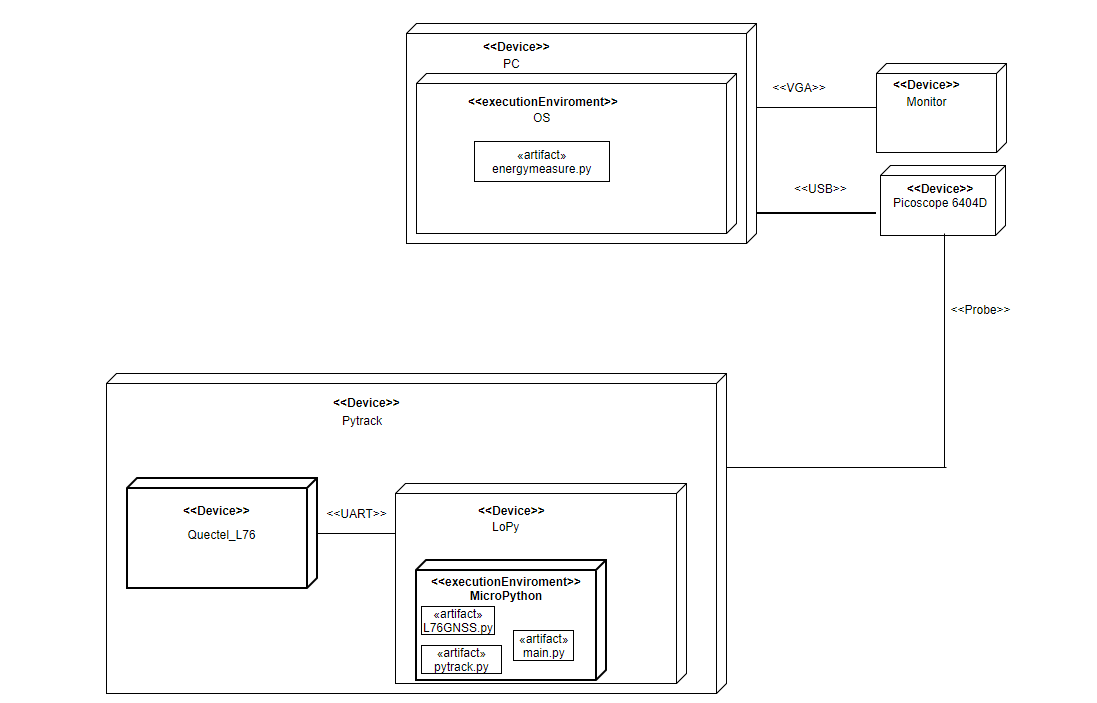
\includegraphics[height=9.5cm]{Project_Report/Images/LoPy_deploy.png}
\caption{Deployment diagram of the LoPy configuration}
\label{fig:LoPy_deploy}
\end{figure}

The LoPy is a microcontroller equipped with a LoRa, Wifi and BLE technology \cite{LoPy} and is specifically made for IoT use cases. It uses the Espressif ESP32 chip and the user write the program code in Micropython. LoPy has a low-power feature which makes it turn off most of the hardware except its internal peripheral. The micro controller has UART, SPI, I2C and up to 24 GPIO.

The LoPy is equipped with Pycom's Pytrack, which is an extension shield to the LoPy. Pytrack is equipped with a L76-l GPS receiver from Quectel and a 3 axis 12 bit accelerometer \cite{Pytrack}. L76-l is a low power GNSS receiver \cite{L76}. The module is equipped with an ARM7 processor and UART for serial communication. The LoPy controls the receiver through the execution of the program code and communicates with the ARM7 processor through serial communication with the Pytrack shield. TTFF for the GNSS receiver is:
\begin{itemize}
\item Cold start:35s
\item Warm start: 30s
\item Hot start: 1s


\end{itemize}


The LoPy offers debugging possibilities over WiFI which enables a simple configuration by measuring the voltage drop directly over the shunt resistor. The schematic of the circuit configuration is shown in \ref{fig:LoPy_Schematic}. The green channel is the common ground for both the red channel and the black channel. The red channel measures the voltage drop over the shunt. The measured signal is inverted in software, because it is referenced to a node that has a higher potential. 

\begin{figure}[H]
\centering
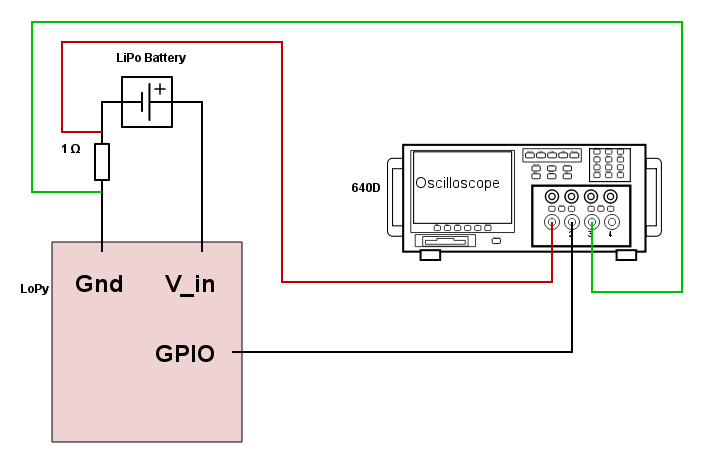
\includegraphics[height=6.5cm]{Project_Report/Images/LoPy_Schematic.png}
\caption{A low side shunt configuration}
\label{fig:LoPy_Schematic}
\end{figure}


\subsubsection{Program code for acquiring a positional fix}
Program code was written for the LoPy. The code was based on the framework published from PyCom. The code initializes the serial communication with the ARM microcontroller on the Quectel L76-l receiver. The next step is to parse the satellite data that is sent from the receiver to the LoPy. The data is sent according to the NMAE protocol. A part of the program code is shown in \ref{code:Parsing of gpsdata}. The code reads the data from serial and tries to find the GPGGA data. The GPGGA contains the fix status and other satellite data. If the GPGGA data is found, the fix status is read and set. The remaining code is included in the appendix \ref{Appendix:L76GNSS.py}

\lstset{language=Python}          % Set your language (you can change the language for each code-block optionally)

\begin{lstlisting}[frame=single]  % Start your code-block

            nmea += self._read().lstrip(b'\n\n')
            .rstrip(b'\n\n')
            gpgga_idx = nmea.find(b'GPGGA')
            if gpgga_idx >= 0:
                gpgga = nmea[gpgga_idx:]
                e_idx = gpgga.find(b'\r\n')
                if e_idx >= 0:
                    try:
                        gpgga = gpgga[:e_idx].decode('ascii')
                        print (gpgga)
                        self.gpgga_s = gpgga.split(',')
                        print(self.gpgga_s)
                        self.get_fix()
                        if(self.fix >0):
                            self.lat_d, self.lon_d
                            = self._convert_coords
                            (self.gpgga_s)
\end{lstlisting}
\label{code:Parsing of gpsdata}









.
\newpage